\chapter{Other Work} \label{gmf}
This chapter explains the work carried out on grahical modeling framework and GrGen and the possibility of using them with current graph rewriting project.

\begin{figure}
 \centerline{
 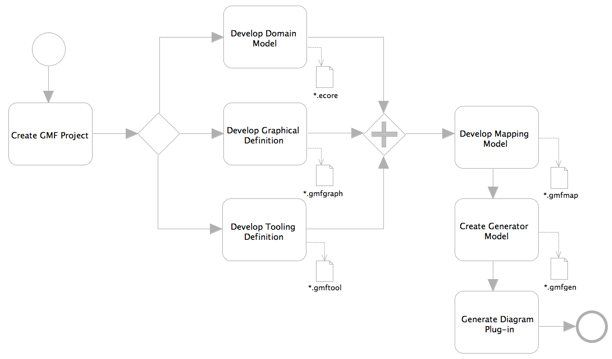
\includegraphics[width=1.0\columnwidth]{figures/gmf.png}
 }
 \caption{Overview of GMF}
 % Quote GMF website
 \label{gmf}
 \end{figure}

\section{Graphical Modeling Project}
The Eclipse Graphical Modeling Project (GMP) provides a set of generative components and runtime infrastructures for developing graphical editors based on EMF and GEF. Since the current graph is built on EMF, it is easy to extend the project to have a graphical editor based on GEF (Graphical Editing Framework). The Graphical Modeling Framework (GMF) Tooling project provides a model-driven approach to generating graphical editors in Eclipse \cite{gmf}.

The GMF runtime is an industry proven application framework for creating graphical editors using EMF and GEF. With these things in picture a graphical editor can be easily created 

\subsection{GMF-Tooling workflow}
The diagram \ref{gmf} illustrates the main components and the work flows of the GMF. 

Once creating the initial project the first task is to create a domain model or use an existing domain model(.ecore). Core to GMF is the concept of a graphical definition model. This model contains information related to the graphical elements that will appear in a GEF-based runtime. An optional tooling definition model is used to design the palette and other periphery (menus, toolbars, etc.). Once the appropriate mappings are defined, GMF provides a generator model to allow implementation details to be defined for the generation phase. The production of an editor plug-in based on the generator model will target a final model. GMF provides this work-flow in eclipse making it easy to generate. 


\section{GrGen}
GrGen (Graph Rewrite Generator) is a software development tool that offers programming
languages optimized for graph structured data, with declarative pattern matching and rewriting at their core, with support for imperative and object-oriented programming, and a bit of database-like query-result processing\cite{grgen}. 

The idea of was to use GrGen for graph transformation. For this requirement was to convert the current graph format(JUNG - Java Universal Network/Graph Framework) to the graph system (explained below) understood by GrGen.NET system and transform the graph and convert it back to JUNG. 

GrGen.NET is fast and efficient but it needs a lot of effort to understand and use it.

Graph is represented using a language called graph modelling language(.gm) and rules are defined in $rule language (.grg)$  with embedded sequences. This rules on the Host graph can be controlled by a Shell script written in GrShell language or  C-sharp application. These can be used for interactive debugging with the graph viewer. 

The central object is the graph, it adheres to the specified graph model. (In general
you have to distinguish between a graph model on the meta level, a host graph created as instance of the graph model, and a statically specified pattern graph of a rule that matches a portion of the host graph at runtime).\\

\begin{itemize}

\item {Reasons for consideration of GrGen.NET}
 
\begin{itemize}
\item GrGen.NET offers processing of graph representations at their natural level of abstraction. It is built on a rich and efficient metamodel implementing multi-graphs, with multiple inheritance on node and edge types. 

\item It reduces the graph transformation hassles(pointer modifications) which existed in low level languages.

\item GrGen.NET is one of the fastest available engines for graph transformation. 

\item Graphs can be exported to .XMI format. XMI files as written by the Eclipse Modeling Framework (EMF) are a standard format in the model transformation community.
\end{itemize}

\item{This project was discontinued because}
\begin{itemize}
\item Converting the graphs in to generic language is very complicated process. Since the idea was to convert any given JUNG graph to GrGen format. It is difficult to write a software that writes a another language. 

\item In the given time frame of the project it was not feasible to complete the work. 

\item The ROI (Return on Investment) was very less.  
\end{itemize}
\end{itemize}


